\PassOptionsToPackage{table}{xcolor}

\documentclass{MScthesisITEM}
\AtBeginDocument{\addtocontents{toc}{\protect\thispagestyle{empty}}} 

% this package is just to generate text for demo-purposes
%\usepackage{blindtext}
\usepackage{listings}
\usepackage{microtype}
\usepackage{tikz}
\definecolor{listinggray}{gray}{0.9}
\definecolor{lbcolor}{rgb}{0.97,0.97,0.97}

\lstset{
    keywordstyle=\bfseries\ttfamily\color[rgb]{0,0,1},
    identifierstyle=\ttfamily,
    commentstyle=\color[rgb]{0.133,0.545,0.133},
    stringstyle=\ttfamily\color[rgb]{0.627,0.126,0.941},
    showstringspaces=false,
    basicstyle=\tiny,
    numberstyle=\footnotesize,
    framexleftmargin=3pt,
    numbers=left,
    stepnumber=1,
    numbersep=12pt,
    tabsize=2,
    breaklines=true,
    prebreak = \raisebox{0ex}[0ex][0ex]{\ensuremath{\hookleftarrow}},
    breakatwhitespace=false,
    aboveskip={1.5\baselineskip},
    columns=fixed,
    upquote=true,
    extendedchars=true,
    frame=tblr,
    backgroundcolor=\color{lbcolor},
}



\title{Power Profiling: From Measurements to Simulation Models} % The title of your assignement; NB use \newlinetitle to start a newline
\author{Terje Runde \&\newline Stian Hvatum} % Your firstname and lastname
\supervisor{Gunnar Tufte, IDI}
\cosupervisor{Asbjørn Djupdal, IDI}

%% Uncomment the following in case you want subfigures; note that there will be a warning for the caption package
 \let\subcaption\undefined
 \let\subfloat\undefined
 \usepackage[bf,hypcap]{caption}
 \usepackage{subcaption}
 \captionsetup{compatibility=false}

\DeclareGraphicsExtensions{.pdf,.jpg}
\graphicspath{{./figs/}}

\loadglsentries{glossary}
\makeglossaries

\begin{document}
\selectlanguage{english}
\pagenumbering{roman}
\pagestyle{plain}

\newcommand{\lstnumberautorefname}{Line}
\newcommand{\algorithmautorefname}{Algorithm}

%% Only for the project
\ifx\frontpage\undefined
\else
    \titleITEM
\fi

%% Only for the master's thesis; for the project report the description is taken from It's Learning and added by the department
% \selectlanguage{english} % Change to 'norsk' if you are writing in Norwegian
% \begin{titlingpage}

\noindent
\begin{tabular}{@{}p{4cm}l}
\textbf{Title:} 	& \thetitle \\
\textbf{Student:}	& \theauthor \\
\end{tabular}

\vspace{4ex}
\noindent\textbf{Problem description:}
\vspace{2ex}

\noindent \Blindtext[2][1]
\vspace{6ex}

\noindent
\begin{tabular}{@{}p{4cm}l}
\textbf{Responsible professor:} 	& \theprofessor \\
\textbf{Supervisor:}			& \thesupervisor \\
\end{tabular}

\end{titlingpage}
% \cleardoublepage

%% There must be an abstract in English, even though the main text is in Norwegian
\selectlanguage{english}
\pagestyle{empty}
\begin{abstract}

\noindent
    * dark silicon \\
    * power wall \\
    * shmac \\
    * good modelling tools \\
    * need for SIMPLE and EARLY STAGE energy estimations \\

    \noindent Since the beginning of semiconductor technology, transistor size has decreased and are still decreasing with a tremendous rate.
This has enabled engineers to build faster and faster single core processors. Faster and more dense processors 

, as there is more space for fancy solutions, and smaller
transistors means shorter switching latencies. In the last couple of years, processors have been kept down by the power wall, which
means that no more power can be dissipated without very clever cooling solutions. This turns out as a lot of space left for transistors
that we cannot use, a phenomenon called dark silicon.






The SHMAC project at NTNU aims to create a heterogeneous computer system that
can make use of dark silicon as space for energy efficient processors and special accelerators. Even though 













\end{abstract}

\cleardoublepage

%% Only for the master's thesis; if the main text is in English and you can write Norwegian, there must be an abstract in Norwegian as well.A
\selectlanguage{norsk}
\pagestyle{empty}
\renewcommand{\abstractname}{Sammendrag}
\begin{abstract}
\noindent Energieffektivitet en av de største utfordringene i moderne
datamaskindesign. Videre ytelsesøkning begrenses av høy strømtetthet, i
tillegg har energieffektivitet stor betydning i alt fra strømregningen på
superdatamaskiner til batterlevetid for små innebygde enheter. I denne
masteroppgaven ser vi nærmere på arkitekturen og energiforbruket til en ARM
Cortex-A9 og lager et verktøy for å forutsi dens strømforbruk gjennom
simulering.

Via målinger og eksperimenter gjort på ekte hardware blir
instruksjonsnivå-strømforbruk bestemt. Videre blir dette koblet til
hendelsesforløp i den samme arkitekturen simulert i gem5.  Verktøyet benytter
disse hendelsene sammen med loggfiler fra simulatoren tol å lage en
representasjon av prosessorens strømforbruk over tid.

Vår metode kan benyttes i prosessorutvikling allerede i simulatorfasen 

\end{abstract}

\cleardoublepage

\selectlanguage{english}% Change to 'norsk' if you are writing in Norwegian

\chapter*{Preface}
\thispagestyle{empty}
This report is submitted to the Norwegian University of Science and Technology
in fulfillment of the requirements for master thesis.  This work has been
performed at the Department of Computer and Information Science, NTNU, with
Assoiate Professor Gunnar Tufte as the supervisor, and Asbjørn Djupdal as
co-supervisor.

Thanks to Gunnar Tufte and Asbjørn Djupdal for all help with the technical work
and the report. Also thanks to Kenneth Sivertsvik, Håkon Øye Amundsen and Joakim
Andersson for help with proofreading the thesis.

\cleardoublepage

\begin{titlingpage}

\noindent
\begin{tabular}{@{}p{4cm}l}
\textbf{Title:} 	& \thetitle \\
\textbf{Student:}	& \theauthor \\
\end{tabular}

\vspace{4ex}
\noindent\textbf{Problem description:}
\vspace{2ex}

\noindent \Blindtext[2][1]
\vspace{6ex}

\noindent
\begin{tabular}{@{}p{4cm}l}
\textbf{Responsible professor:} 	& \theprofessor \\
\textbf{Supervisor:}			& \thesupervisor \\
\end{tabular}

\end{titlingpage}
\cleardoublepage
% similarly you may add a separate acknowledgments page

\tableofcontents*
\cleardoublepage

%% include if relevant
%\listoffigures
%\cleardoublepage

%% include if relevant
%\listoftables
%\cleardoublepage

%% include if relevant
%\listofalgorithms
%\addcontentsline{toc}{chapter}{List of Algorithms}
%\cleardoublepage

%% include if relevant
%\printglossary[title=List of Symbols, style=long]
%\cleardoublepage
%\glsaddall[]

%% include if relevant
%\printglossary[title=List of Acronyms,type=\acronymtype] % prints just the list of acronyms
%\cleardoublepage

\pagenumbering{arabic}
\pagestyle{ruled}
\chapter{Introduction}

This thesis looks into many aspects regarding prediction of energy consumption
on both existing and non-existing hardware. Methods for mapping power
consumption to specific events at the architectural level are looked into.
Further, a program that leverages modern architectural simulators for
power-aware hardware development are being created and evaluated.

\section{Motivation for energy efficiency}
% Moore, blabla Amdahl, blabla Pollac, blabla other people.

During the 90's and early 2000's, single-threaded performance doubled every 18th month. As more performance
was crammed into larger and larger cores, heat and power consumption became overwhelming. To remedy this,
more recent designs has put a lot of effort into making the processor energy efficient.


\section{Assignment Interpretation}

Based on the assignment description text, the following main tasks were
identified.

\begin{description}
    \item[Task 1:] Quantify the exact cost of executing specific instructions on
        a modern out-of-order CPU core
    \item[Task 2:] Create a software suite that sheds light on the energy
        consumption during software execution on various hardware
\end{description}

As can be seen, the problem is twofold. \textit{Task 1} involves performing energy
measurements on hardware components to obtain numbers of a processors energy
characteristics. \textit{Task 2} depends on the results from the former and can
be solved after the completion of \textit{Task 1}.

The first task was solved as a part of the specialization project (TDT4501)
during the fall of 2013, and the final report in its entirety is attached in
\autoref{RH13}. The review of \textit{Task 2} is the main emphasis of this
master's thesis.

\section{Related Work}

Butko et. al.\cite{butko2012accuracy} evaluated the accuracy of the gem5
simulator against a Snowball SKY-S9500-ULP-C01 containing a dual core 1GHz ARM
Cortex-A9.  Their work reports very good accuracy for benchmarking workloads,
with runtime accuracy reported between 1.23\% and 35.31\%.  Most of the tests
were well within 6\% mismatch, but the tests containing a high number of
L2-misses had a high runtime discrepancy between hardware and simulation. Butko et. al.
utilized the SimpleTiming CPU model and the basic memory system of gem5.

Pusderis et. al. \cite{pusdesrissources} evaluated errors in full system
simulation using gem5, and found that with proper modelling of the CPU model
and memory system, they got a mean runtime error of 17\% when running the PARSEC
test suite and 13\% running SPEC CPU2006. Their research is based on a ARM
Versatile Express TC2 development board containing an ARM Cortex-A15, a modified
ARM Out-of-order CPU model for gem5 and some adjustments to the memory model.

This work is based on Runde et. al.\cite{rundehvatum2013exploring} where isolated
power drain of different instructions where measured.

\begin{enumerate}
    \item SimplePower (Penn State)
    \item McPAT (HP-Labs)
    \item PowerAnalyzer (University of Michigan)
    \item Wattch (Princeton)
    \item LLVM Energy Models
\end{enumerate}

\section{Report Organization}

%TODO: Verify that the section titles here are similar to the real titles.

\begin{description}
    \item[Chapter 1: Introduction] provides a historical perspective to the
        trends in processor design and motivates the need for energy efficient
        hardware.
    \item[Chapter 2: Background] contains background material on topics touched
        in this thesis, as well as explanations that support decisions made
        later in the report.
    \item[Chapter 3: Building a Power Estimation Tool] is the main piece of our
        problem solution. It contains an in-detail review of what PET does and
        how it is built.
    \item[Chapter 4: PET Performance Tuning] describes what one must consider
        when porting the use of PET to support new hardware configurations.
    \item[Chapter 5: Experiments and Results] presents the test setup and
        performance obtained from our experiments.
    \item[Chapter 6: Conclusion and Further Work] provides the concluding remarks on the work
        described in this thesis and suggests possible areas of interest for
        further research.
\end{description}



\chapter{Background}
\input{background/power_est.tex}
\chapter{gem5 Accuracy}

A key to high accuracy power estimation is a high accuracy architectural
simulator. Without a simulator capable of providing decent accuracy over system
events, power estimation using methods as suggested in this report will fail.
There exists related work that claims a very high accuracy for
gem5\cite{butko2012accuracy,blem2013detailed}, but the results states
good accuracy for benchmark programs with a high diversity of instructions. A common
factor for much of this related work is that the benchmarks have been run with
simple CPU models that are single cycle and in-order, but timing-adjusted to fit
the performance of the real hardware.

The power estimation scheme suggested in this thesis is based on accumulation of discrete
events, each with an assigned weight related to its contribution of the global power consumption.
This means that accurate power estimation needs these discrete events to happen, and they must
happen with a realistic timing related to their triggering cause. This chapter will dive into
how well gem5 does this, but also problems that one must be aware of when using gem5 or any
other simulator this way.


\section{CPU Modelling in gem5}

The revision of gem5 used for these experiments, changeset aaf017eaad7d,
contains a decent model for the ARM Cortex-A9 processor. Actually, the
implemented CPU is a generic out-of-order processor capable of running the ARMv7
ISA, which is equal to that of ARM Cortex-A9\cite{armtech}. The performance of
the ARM Cortex-A9 will differ between its implementations, and to make it even
harder, most vendors will not disclose details to the public. It has been
discussed among the gem5 users wherever the default configuration for this
processor actually is equal to any real processor\cite{a15maillist}, but the
general answer is that no one knows or are allowed to tell.

The goal of this project it to be able to estimate power for new architectures
that might or might not be close to existings architectures, but as a reference
for the implementation, a good model for a known processor is needed. The
hardware platform and the experimental setup is equalt to that in
\cite{rundehvatum2013exploring}, so gem5 must be adapted to simulate a Samsung
Exynos 4412P, or at least the CPU-part of it.  gem5 is made to be adapted, so
adaption is mostly done through editing python files. A new file was created in
\texttt{gem5/configs/common/Exynos\_4412P.py} and a few others where edited to
include this new processor definition. The processor definition used and other
modifications done to the original changeset aaf017eaad7d can be found in
\autoref{apx:gem5files}.

As a decent amount of implementation details often are keept secret from end users, it
is not trivial to model any commercial processor. To get as equal as possible performance
and event scheduling to the real hardware, parameters was fetched from around the internet,
and the simulator was then scripted to run with a wide variaty of configurations and
mutations of these, all for the ARM Out-of-order CPU model. When the run time performance was
as good as time permitted, the configuration was accepted and used further in the experiment.
This final configuration is the one printed in \autoref{gem5exynos4412p}. Sources suggesting
parameters for ARM Cortex-A9 or Samsung Exynos 4412P is listed in \autoref{fig:a9paramsources}

\begin{figure}
All web references was found between january and april 2014.
\begin{itemize}
    \item{\cite{blem2013detailed}}
    \item{\cite{butko2012accuracy}}
    \item{\cite{armtech}}
    \item{\url{http://en.wikipedia.org/wiki/Odroid}}
    \item{\url{http://en.wikipedia.org/wiki/Exynos}}
    \item{\url{http://www.geekland.co/ARM-Cortex-A9-Exynos-Quad-Core-4412-Android-Development-Board-GK-4412P.htm}}
    \item{\url{http://www.7-cpu.com/cpu/Cortex-A9.html}}
    \item{\url{http://www.arm.com/products/processors/cortex-a/cortex-a9.php?tab=Specifications}}
\end{itemize}
\caption{Sources suggesting parameters for ARM Cortex-A9 or Samsung Exynos 4412P}
\label{fig:a9paramsources}
\end{figure}

\section{gem5 Accuracy}



\begin{table}
\centering
\begin{tabular}{|l|c|c|c|c|}
\hline
 & add-add & pi-pi & sha2-sha2 & trend-trend \\
\hline
Real hardware & 0.017600  & 0.013500 & 0.022600 & 0.014600 \\
gem5 modified O3    & 0.017541  & 0.013790 & 0.022819 & 0.011898 \\
gem5 original 03    & & & & \\
gem5 timing simple & & & & \\
\hline
\end{tabular}
\caption{gem5 runtime accuracy (O3 with classic memory system)}
\label{tbl:gem5runtimeaccuracy}
\end{table}



\input{background/ga.tex}

\chapter{Building a Power Estimation Tool}

The ultimate goal for this project is to model and estimate energy consumption
for not yet implemented computer architectures. This allows new ideas to be
prototyped and evaluated with respect to energy efficiency already at the design
stage, easing the process of building energy efficient hardware. These
evaluations can only serve as estimates and will doubtedly be truly accurate.
Nevertheless, it can be used to test specific workloads and applications on
specific processor configurations and evaluate ideas rapidly during the design
phase.

As we are already supplied with a computer architecture simulator capable of
tracing all sorts of hardware events, the next step is to extract power
information from these event logs. In this chapter we introduce PET, a Power
Estimation Tool. PET provides guided information about power usage for computer
architectures and represents a major piece of our problem solution. The chapters
to follow describe how it works along with its strengths and weaknesses.

\noindent PET is implemented in C++ using the Boost Library \cite{boostwebpage}. The source code for
PET and the rest of this project can be found at Github:

\begin{lstlisting}[language=bash,numbers=none]
git clone https://github.com/terjr/thesis.git
\end{lstlisting}

\section{Concept}
The goal for PET and this project is to ultimatly estimate power usage and thus
also energy efficiency of still not yet implemented computer architectures. A
such approach will of course reside well within the term "estimation" and will
doubtly reach the correct numbers. Never the less, PET is built by measuring
real hardware with great detail, capturing discrete events and assigning each
event a certain amount of energy consumption.

As depicted in \autoref{fig:workflow}, when selected events have been weighted,
one can run the test program though a simulator set up to act as the new
hardware.  The simulator will generate a tracelog containing the weighted
events, and PET can then apply the numbers. From this workflow, PET can produce
a data set containing power consumption distributed over the simulation
lifetime.  As noted, the new hardware will be weighted equally of a chosen
existing hardware, so so this method requires a certain similarity beteen the
new and the old hardware. In general, all traditional architectures contains
equal principles of function, and is thus mappable to each other, but accuracy
will of course differ as hardware differs in design, applied voltage, clock
speed and process technology.

\begin{figure}
    \includegraphics[width=0.9\textwidth]{figs/pet-workflow-gv.pdf}
    \caption{Workflow using PET}
    \label{fig:workflow}
\end{figure}

When estimating power usage for new architectures, it is hard to tell exactly
how to chose events and how expensive each event is. Therefore, we have to
assume that the new architecture is comparable to an old architecture, and thus
we can use the same power estimation numbers to give a new estimate.

\section{Approach}

While HDL-languages as well as computer architecture simulators have been around
for quite some time, energy estimation techniques is a more recent necessity.
Song et. al \cite{song2012instruction} identifies three major approaches to
processor power modelling used in the past, and introduces an instruction-based
energy estimation model that can be used for energy simulation at high speed.
Their proposed method is expressed through the following equation and includes
the desired features of past energy models.

\[
    P_{core}(t) = \frac{E_{unit} \cdot A_{datapath} \cdot w(t) +
    E_{static}}{T_{sampling}}
\]

This method depends on two things. First, one must know sufficient details of
the processor to identify datapath components in order to form the
$A_{datapath}$ matrix. Secondly, the energy unit vector $E_{unit}$ requires
circuit-level knowledge of the target processor. The former information can
often be found by reverse engineering and benchmarking, however, the latter is
rarely available for commercial processors. When building the model for PET, we
simplify the model from \cite{song2012instruction} by combining $A_{datapath}$
and $E_{unit}$ to form a vector of weights that directly corresponds to the cost
of an event. We can then model energy by the following formula.

\[
    P_{core}(t) = \frac{C \cdot w(t) + E_{static}}{T_{sampling}}
\]

Here, C represents the global cost vector -- a matrix enumerating the cost
for all event types. Please note that it is global and do not depend on time.

\subsection{Power Consuming Events}
\label{subsec:powerevents}

The choice of events/workload metrics is an important part of our method. We
account for two types of events; CPU instruction events and memory activity
events. It is desirable to estimate energy consumption on literally all types of
computing systems, ranging from large-size clusters to embedded systems. To
provide this flexibility it was decided that PET should parse log files from the
simulators rather than being built-in on a chosen simulator.  Most active and
working architectural simulators supports this sort of trace logs, and even if
they are formatted different, the effort of adjusting to a new format is a lot
less than the effort of building this tool within even another simulator.

The trace logs contains information about everything that goes on within the
fictional computer, and thus PET can extract useful information from this log
file. A piece of such useful information is defined in PET at a \emph{simulator
event}. A simulator event can be thought of as a unit of work that uses a
specified amount of energy. When PET finds such an event, it increases the
modelled energy consumption along the timeline at the time the event took place.

\begin{table}[ht]
    \centering
    \begin{minipage}[b]{\linewidth}
        \centering
        \begin{tabular}{|l|l|}
            \hline
            IntAlu    & Integer basic ALU operation\\
            \hline
            IntMult    & Integer multiply ALU operation \\
            \hline
            MemRead    & Memory Read issued, triggers LS-unit \\
            \hline
            MemWrite    & Memory Write issued, triggeres LS-unit \\
            \hline
            SimdFloatMisc     & NEON-unit activated \\
            \hline
        \end{tabular}
        \subcaption{CPU Core Events}
    \end{minipage}

    \begin{minipage}[b]{\linewidth}
        \centering
        \begin{tabular}{|l|l|}
            \hline
            L1IR    & L1 instruction cache, read \\
            \hline
            L1IW    & L1 instruction cache, write \\
            \hline
            L1DR    & L1 data cache, read \\
            \hline
            L1DW    & L1 data cache, write \\
            \hline
            L2R     & L2 cache, read \\
            \hline
            L2W     & L2 cache, write \\
            \hline
            PhysR   & Main memory, read \\
            \hline
            PhysW   & Main memory, write \\
            \hline
        \end{tabular}
        \subcaption{Memory Events}
    \end{minipage}
    \caption{Power Consuming Events}
    \label{tbl:events}
\end{table}

The events which PET recognizes are briefly described in \autoref{tbl:events}.
These events are chosen mainly based on what information that is easily
extracted from a gem5-formatted trace log, but also adjusted by what information
we could check with performance counters without a very high amount of effort.
Most of this information is available from \cite{rundehvatum2013exploring},
where different instruction loops where measured with both ammeter and
performance counters. This is then correlated with \autoref{fig:a9arch} which
gives an architectural overview of the CPU core where different parts of the
pipeline is visible.

\begin{figure}
    \centering
    \includegraphics[width=\textwidth]{figs/A9-Pipeline-hres.jpg}
    \caption{A brief overview of the Cortex A9 Pipeline, figure from the ARM Cortex-A9 Whitepaper \cite{a9whitepaper}}
    \label{fig:a9arch}
\end{figure}

\section{Input}
New hardware architectures are not easily analysed without physical
implementation, but often we are able to simulate its behaviour to acceptable
accuracy, and thus we are able to test different implementations with low cost.
These simulation runs can often be set up to produces trace logs which contains
a user controlled amount of detail. PET can use these trace logs and scan them
for predefined events, each affecting the power consumption of the simulated
hardware. Different simulators have different trace log formats and different
trace abilities. We have chosen gem5 as our target simulator as it is easy to
configure, and trace is well implemented. As mentioned in
\autoref{subsec:design_choises} other options are available, but the support for
easily configurable CPU- and memory system along with the pre-implemented ARM
processors and in-department hands-on experience with this simulator made gem5
the most logical choise.

\subsection{gem5 trace logs}
When run with \texttt{--debug-flags=Bus,Cache,MemoryAccess,Exec} gem5 will output trace files look like
the text displayed in \autoref{lst:trace}.

\begin{lstlisting}[basicstyle=\tiny,caption={gem5 trace log},label={lst:trace},escapeinside={@}{@},float]
@\label{line:physmem}@3021: system.physmem: Write of size 8 on address 0x82fe0 data 0xe1a0f00eee1d0f70
@\label{line:icache}@3021: system.cpu.icache: access for ReadReq address 9c0 size 64
@\label{line:cachemiss}@3021: system.cpu.icache: ReadReq (ifetch) 9c0 miss-
...
@\label{line:cacheupdate}@3432: system.cpu.dcache: Block addr 81f0 moving from state 0 to state:7 valid: 1
3432: system.cpu.dcache: Leaving recvTimingResp with ReadResp for address 81f00
3432: system.tol2bus.respLayer1: The bus is now busy from tick 234320 to 236376
@\label{line:memread}@1642: system.cpu T0 : 0x89d4.0 : ldr   r1, [sp] #4     : MemRead :  D=0x00000000
@\label{line:intalu}@1642: system.cpu T0 : 0x89d4.1 : addi_uop   sp, sp, #4 : IntAlu :  D=0x00000000b
1701: system.cpu T0 : 0x89d8   : mov   r2, sp          : IntAlu :  D=0x00000000b
1701: system.cpu T0 : 0x89dc.0 : str   r2, [sp, #-4]!  : MemWrite :  D=0x0000000
1760: system.cpu T0 : 0x89dc.1 : subi_uop   sp, sp, #4 : IntAlu :  D=0x00000000b
1760: system.cpu T0 : 0x89e0.0 : str   r0, [sp, #-4]!  : MemWrite :  D=0x0000000
4000: system.membus: recvTimingResp: src system.membus.master[0] ReadResp 0x1640
4000: system.l2: Handling response to ReadResp for address 1640
4000: system.l2: Block for addr 1640 being updated in Cache
\end{lstlisting}

Each line in \autoref{lst:trace} represents an event that happens in the
simulated hardware.  \autoref{line:physmem} tells that a write access to
physical memory has happened. \autoref{line:icache} is the event of instruction
cache access, while \autoref{line:cachemiss} shows that this request failed.
During this simulation, there is also events like \autoref{line:cacheupdate}
which represents that the data cache updates some content. The discrete
instructions running through the CPU is also logged, eg. \autoref{line:memread}
shows a load-instruction and \autoref{line:intalu} shows an
addition-instruction.

As discrete events are picked out from the trace logs, PET accumulates power
consumption in equally sized timeslots, called buckets. Each bucket has a
parameter controlled size in terms of simulator ticks. Often it is more
practical to specify the number of buckets in the output rather then specifying
the number of simulator ticks in each bucket. Because of this, PET is able to
estimate the bucket size by peeking at the tick at the last line of the trace
file. It has been shown that the trace file is not nessesary in tick order,
but it will commonly be at approximatly the last tick at the last line. The
bucket size estimation algorithm is shown in \autoref{alg:bucket_size}.

\begin{algorithm}
    \caption{Bucket Size Detection Algorithm}
    \label{alg:bucket_size}
    \begin{algorithmic}
        \Function{numTicks}{$traceFile$}

        \State $eofPos \gets \Call{getSize}{traceFile}$
        \State $\Call{seek}{traceFile, eofPos - 3}$
        \State
        \State $char \gets \Call{getChar}{traceFile}$
        \While{$char \ne newline$}
            \State $\Call{seek}{traceFile, -1}$
        \EndWhile
        \State $line \gets \Call{getLine}{traceFile}$
        \State $simulatorEvent \gets \Call{parseLine}{line}$
        \State \Return $\Call{getTick}{simulatorEvent}$
        \EndFunction
    \end{algorithmic}
    \begin{lstlisting}[language=Python]
function numTicks( traceFile ):
    # Find file size
    eof_pos = traceFile.getSize()

    # Seek almost to end, avoid last newline
    traceFile.seek( eof_pos - 3 )

    # Trace from back of file to second last newline
    while not traceFile.currentChar is '\n':
        traceFile.seek_backwards

    # File stream position is now at beginning of last line
    # Parse this line
    simulatorEvent = parseLine( traceFile.getLine() )

    # Return the tick of the retreived event
    return simulatorEvent.getTick()
    \end{lstlisting}
\end{algorithm}

\autoref{lst:trace} also shows that the events in the trace log is not nessesary in their
correct order, thus PET has to be able to add power consumption to the entire timeline at all
time. This means that we are unable to produce continous output, but have to store the
results in memory and dump them when the entire input is parsed.


\subsection{PET weight files}
Equally important as finding the correct events is assigning each event the
correct amount of power consumption. As each event will count differently
depending on the architecture, PET will read a weight file along with the gem5
trace log. A sample weight file is listed out in \autoref{lst:weights_example}.
As the timeslots are specified in simulator ticks instead of CPU cycles,
the values have been chosen to match a 2GHz processor, which then means
one CPU cycle pr. 500 simulator ticks using standard gem5 simulation granularity.
If you are applying this method to a processor with a different clock speed than
2GHz, be aware that the numbers has to be scaled propotionally. This is not the
case for the static power drain, as it is simply added to each timeslot, and is
not scaled in accordance with bucket size.

\lstinputlisting[caption={Weight file example},label={lst:weights_example},float,language=Python]{examples/weights.conf}

The weights displayed in \autoref{lst:weights_example} are assigned and
accumulated each time PET discovers a recognisable event in the log file. A
simplified version of this algorithm can be found in
\autoref{alg:power_accum_algo}

\begin{algorithm}
\caption{Power Accumulation Algorithm}
\label{alg:power_accum_algo}
\begin{lstlisting}[language=Python]
# map of accumulated power for each time step
map<time,power> output

# input is all trace log lines, elements in weight file and
# the determined bucket size (number of simulator ticks in
# each bucket)

function assignWeights( traceLogLines, weightMap, bucketSize )
    # run through each line
    for each line in traceLogLines:
        # extract event parameters from line
        simulatorEvent = parseLine( line )

        # get the assigned weight from weight file
        eventWeight = weightMap[simulatorEvent.getEventType()]

        # add this weight to the output map
        output[simulatorEvent.getTick()/bucketSize] += eventWeight
    return output
\end{lstlisting}
\end{algorithm}
%weightfiles
%

\subsection{Annotation files}
\label{subsec:annot}
PET has the ability to annotate it's output using a map from PC to function name. The
simulated binary itself is not an input to PET, as it would contain to much information to display nicely in
an ordinary graph. Instead, PET comes along with a tool called \texttt{scripts/annotate.sh} which takes
a binary file as input and prints out all function names in the binary file. The binary file must be compiled
with debugging symbols for this to work. The usual situation would then be to pull out those function names you want
to annotate be editing the output from this tool, and then giving this file to PET as annotation input.

An example of how this map can look like is printed in \autoref{lst:annot}. The
left column is simply the PC value where the function label points, and the
right column is the function name.
\lstinputlisting[caption={Annotation file example},label={lst:annot},float,language=Python]{examples/annot.conf}

\section{Output}
\label{sec:output}

When a log file is consumed by PET, the output should be usable for many
applications. In early stages of the design phase, or when great differences are
expected, a sparse annotated graphical output might be the best way of
visualizing power consumption. As the project evolves and more subtle changes
are evaluated, a textual output will be easier to compare. PET supports three
different output options:

\begin{description}
    \item[graph]\hfill\\
        This format is the default, and provides an overview of
        the entire program in an easily digestible format. An example of such
        a graph is printed in \autoref{fig:annot}.
    \item[plain]\hfill\\
        The example in \autoref{lst:pet_output_plain} shows the \emph{plain}
        format, which is intended to be used for further machine processing.
    \item[table]\hfill\\
        The table format, with an example shown in
        \autoref{lst:pet_output_table}, shows a terminal-printable output which
        is easier to read. It might come in handy as the default format might be
        hard to read when you are looking for specific information.
\end{description}

\subsection{Units}

The output format is understood as timeslots in which the architecture has a
certain current drain, which should be multiplied with applied voltage to get
consumed energy. The values are given as milliamperes, equal to milliwatt if
voltage is $1~V$. Milliamperes are used as it is easier to find current drain
rather than wattage with the setup used in this project, as described in
\autoref{sec:energymeasure}. When power is estimated for a new architecture, the
resistance of the circuit is difficult to deduce, and voltage might also be an
unknown factor. Given Ohms law in \autoref{eq:ohm} and the definition of
electric power in \autoref{eq:power}

\begin{equation}
I=\frac{U}{R}
\label{eq:ohm}
\end{equation}

\begin{equation}
P=U \cdot I
\label{eq:power}
\end{equation}

it can be found that power equals current squared times resistance

\[U=R \cdot I\]
\[P=(R \cdot I) \cdot I\]
\begin{equation}
P=I^2 \cdot R
\label{eq:currentsquared}
\end{equation}
and that power equals voltage squared divided by resistance
\[P=U \cdot \frac{U}{R}\]
\begin{equation}
P=\frac{U^2}{R}
\label{eq:voltagesquared}
\end{equation}

Thus, estimating only the current drain means that the power at each point will
be unknown without knowing resistance or voltage. Further, energy consumption
cannot be estimated unless the new architecture is similar in terms of voltage
and resistance to a chip where these numbers are available. Even the current
drain might not be representable at all; if resistance or voltage is unequal to
the levels found in the reference chip, the final numbers will be far off.

\autoref{eq:currentsquared} and \autoref{eq:voltagesquared} states how voltage
and current is important for energy consumption. The current is, from
\autoref{eq:ohm}, dependent on resistance as well as voltage. With this in mind,
and knowing that power in a complex environment is a delicate matter, the most
important application for PET is to point in the right direction. PET will never
give accurate power estimations for new chips, but will provide useful
information for seeing if a new feature or architectural fix will render the
final architecture more energy efficient or not.


\subsection{Examples of Output Data}

Visualization is often a good thing when inspecting old or trying to understand
new problems. \autoref{fig:annot} shows an example of PET \texttt{graph} output
format, with annotations.

\begin{figure}[htb]
    \centering
    \includegraphics[width=0.9\textwidth]{figs/annot.pdf}
    \caption{PET graphical output. This example contains annotations, each label
    represents the entrance of a function.}
    \label{fig:annot}
\end{figure}

Example of the \texttt{plain} output format can be seen in
\autoref{lst:pet_output_plain}. The left column is the bucket number, while the
right column is instant current draw from the modeled architecture.

\begin{lstlisting}[numbers=none,float=hbt,label={lst:pet_output_plain},caption={PET plain output with function annotations.}]
0 120 memcpy
1 113 start
2 150 main
3 123 main
4 133 fun1
5 117 main
\end{lstlisting}

When reading the output directly from console, a more descriptive output format
is the \texttt{table} format. An example using this option is rendered in
\autoref{lst:pet_output_table}.

\begin{lstlisting}[numbers=none,float=hbt,label={lst:pet_output_table},caption={PET table output with function annotations.}]
/----------------------------------------\
|   Bucket   |  milliAmps |    Symbol    |
|------------|------------|--------------|
|          0 | 120.000000 |    memcpy    |
|          1 | 113.000000 |    start     |
|          2 | 150.000000 |    main      |
|          3 | 123.000000 |    main      |
|          4 | 133.000000 |    fun1      |
|          5 | 117.000000 |    main      |
\----------------------------------------/
\end{lstlisting}



\section{Architecture}

Modern computer science emphasize parallelism as a highly important property in
order to achieve speed on multicore processors. As the size of the log files
which PET has to parse can easily be 10s of gigabytes large, PET has to be
designed with performance in mind. This means that PET must be lightweight and
parallel in order to be fast, while it must maintain correctness and be easy to
use.

Due to memory constraints on commonly available computers, it is not feasible to
read the entire log file into memory and then start parsing. It would also make
the reading step a serial part of the program, which hinders parallelism. It
will also be a bad idea to read one line, parse it, weight it and apply it to
the grand total, as it would be an entirely serial process.

\subsection{Overview}

\begin{figure}[ht]
    \includegraphics[width=0.9\textwidth]{figs/pet-pipeline-gv.pdf}
    \caption{How PET works}
    \label{fig:pipeline}
\end{figure}

In order to maintain good speed while still keeping the PET source code
readable, we have looked at different ways of chewing through large data sets.
The final implementation of PET follows a scheme borrowing ideas from the
producer-consumer patterb as explained by Gamma et. al. in \cite{designpatterns}
and the MapReduce algorithm \cite{dean2008mapreduce}. As depicted in
\autoref{fig:pipeline}, this scheme makes it rather easy to let a producer read
the lines from the log file into ring buffers (produce) and let multiple
consumers pick from each their ring buffer (consume). Each consumer parses the log
lines they pick, and apply the weight of each read event to each their result
vector (map). When all lines are read and parsed, the results vectors are
merged, and idle-task power and static power consumption is added (reduce). This
combination of algorithms allows PET to take advantage of as many cores as
possible, limted only by how fast the producer can read the log files. Finally,
a human readable output is produces, either as a gnuplot line graph or as
formatted or plain text output.

The next subsections will describe in detail the most imporatant parts of the
workflow. For further understanding of the program flow, a call graph extracted
from the entire source code can be found in \autoref{fig:callgraph}.

\begin{figure}
    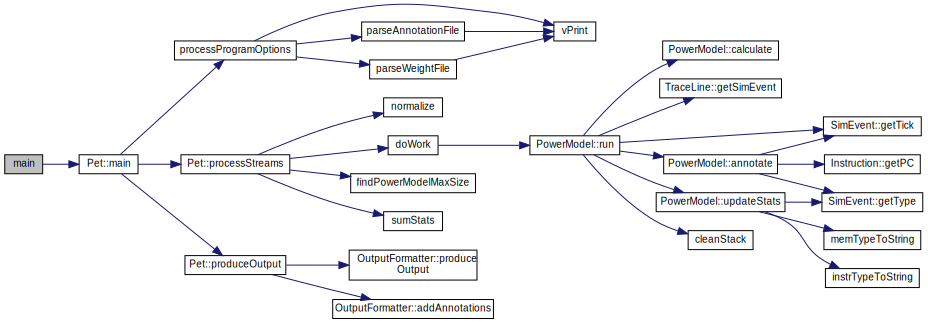
\includegraphics[width=\textwidth]{figs/maincallgraph.pdf}
    \caption{Call graph}
    \label{fig:callgraph}
\end{figure}



\subsection{Argument Parsing and Program Options}

As any other non-trivial programs, PET has to adapt to input options given from
the command line or from a settings-file. PET makes extensive use of the
\texttt{Boost}-library \cite{boostwebpage} and utilize
\texttt{Boost::Program\_options} for parsing the command line. Making use of
\texttt{Boost} for common tasks all over the program made the development cycle
less cumbersome and more rapid. \texttt{Boost::Program\_options} allows easy
extraction of program options, both with long (\texttt{\textemdash \textemdash
option=\emph{value}}) and short (\texttt{\textemdash o~\emph{value}})option
style.


\subsection{Reading Trace Logs}

When arguments are parsed and a trace log has been specified, either by path or
as \texttt{stdin}, a single thread is kicked off reading each line of the log
file into a C++ string container. This happens in the
\texttt{Pet::processStreams} method seen in \autoref{fig:callgraph}. The string
container is then inserted into one of many circular buffers. The circular
buffers are implemented with \texttt{boost::lockfree::spsc\_queue}, a lock free
single producer, single consumer queue. The property of beeing lock free is
explained by Tim Blechmann and the boost-community in \cite{boostlockfree} as
follows: "data structures are \emph{lock-free}, if some concurrent operations
are guaranteed to be finished in a finite number of steps. While it is in theory
possible that some operations never make any progress, it is very unlikely to
happen in practical applications". In PET, this queue has a fixed size of 8192,
but dynamic size is also available in the library implementation.

Which buffer the string is inserted into is determined by a simple circular
algorithm; the next ring buffer is selected when current one is full. When the
buffers are small enough to be filled fast enough to let all workers do work,
this method creates a lot less locking than using a single ring buffer shared by
all worker threads. The number of threads and the size of the ring buffers are
tightly coupled with how fast the host computer is able to feed PET with the log
files.

It is our experience that reading the log file is not the bottle neck, and it is
easy to feed at least 8 cores when the log file is hosted on a reasonable fast
drive. A simple benchmarking done with PET running on a system consisting of an
Intel Core i7 4820, 32GB DDR3 SDRAM and keeping the log files on a fake-RAID
Level-0 consisting of two Western Digital Caviar Black 750GB disks shows this.
PET running with 8 threads on this particular system is consuming the log files
with a rate of 133MB/s regardless of where the log files resides in RAM or on
disk. The benchmark used a log file of 5458MB and was run in 40.871 seconds.

\subsection{String to Event Mapping and Power Accumulation}

String parsing and mapping resembles the most compute-intensive parts of PET.
These parts of the program is kicked off as thread starting the
\texttt{doWork}-function, as the thread library cannot start running in methods
of instanceiated objects. As displayed in the callgraph in
\autoref{fig:callgraph}, this function simply starts the
\texttt{PowerModel::run}-method on its input, which an instance of the
PowerModel-class.

As the producer fills the ring buffers for each of the workers, the workers pick
strings from their pool. The strings are popped from the ring buffer, thus
making space for new elements right away. Each string is parsed by the TraceLine
class, which looks for patterns in the strings containing known event types.
When connecting PET with gem5, the trace logs as previously seen
\autoref{lst:trace} contains an event type designation in the second :-separated
column. The TraceLine class extracts this part using a very simple method to
make this part go fast, outline of this method is listed in
\autoref{alg:extract}.

\begin{algorithm}
    \begin{lstlisting}[style=algo,language=python]
function extractEventType( line ):
    start = line.find(":") + 1
    end = line.find(":", start)

    while (line[start] == ' ')
        start = from + 1
    while (line[end-1] == ' ')
        end = to - 1

    return line.substring(start, end)
    \end{lstlisting}
    \caption{Event Type Extraction}
    \label{alg:extract}
\end{algorithm}

In the real program, some more error handling is present, and the event types
are instanceiated as objects of their parent type (Instruction- or
Memory-event). The right parameters are further found from progressive string
parsing. If the event is not recognized, an "empty" object of type UnknownEvent
is returned, this type always has zero weight. Each event object is able to
figure out its own weight as written in the \emph{weights}-file. After the
event has been parsed, its weight is added to the power model at the right
time step.

In order to reduce the time used for disposal of the string objects
after they are parsed, they are places in a static-size array. When
this array is full, or the ring buffer is empty, the worker deletes
all the strings in a chunk. This methods keeps the memory footprint
low while not calling \texttt{free()} at a continuous rate. The \texttt{free()}
function is not considered very slow, but from the reference implementation
shown in \cite{kernighan1988c}, it does contain enough pointer
arithmetics to make a difference in a tight loop.

\subsection{Data Reduction}

When all lines from the trace log are consumed by the workers, the threads are
joined and their data is returned as standard C++-vectors. These result vectors
are further wrapped in yet another standard C++-vector. The inner vectors is
then looped over together, and the value from the current data point in each
vector is added together and put in a result vector. This accumulation happens
as the last part of \texttt{Pet::processStreams} as seen in
\autoref{fig:callgraph}. After a single point has been accumulated from the
vectors, idle time is calculated from how many events that was recorded during
the data point. This is done more simplistic than accurate using
\autoref{eq:idle}. $numEvents$ is the number of events recorded in each vector
at each measure point, and each event is pinned to the cycle where it
originated.

\begin{equation}
    totalEvents = \sum_{n=1}^{N} numEvents_n
\end{equation}
\begin{equation}
    idleEvents = \frac{ticksInDatapoint}{ticksInCycle}- totalEvents
\label{eq:idle}
\end{equation}

It should be noted that even though this method might work well in a
single-cycle in-order CPU, the out-of-order nature of the Cortex-A9 makes it
hard to tell how much idle time actually exists. E.g. A single cycle may fill
the pipeline with four events, then idle the three next cycles; this would be
calculated as no idle time. When the approximate numbers of \texttt{idleEvents} have been
estimated, that number is multiplied by the \emph{Idle}-weight and added to the
sum in the result vector. Finally, the entire vector is normalized according to
bucket size and then static current drain is applied.


\subsection{Output Production and Annotations}

After the result vector has been completely accumulated, annotation
is added to a new result vector in the same manner as the data reduction.
With the new, merged annotation map containing all last matches between
a symbol and the program counter within each measure point, this map
is feed to the \texttt{OutputProducer}-object as seen in \autoref{fig:callgraph}.
The \texttt{OutputProducer}-object is responsible for generating output as defined
by the input arguments. Its options have already been described in \autoref{sec:output},
and its implementation is a simple nested if-else-clause that calls internal functions for
each output type. The graphical output is produced using a wrapper around GNUPlot, while
the textual outputs are created by \texttt{printf}-statements.


\subsection{Unit Tests}

All internal string parsing are verified by unit tests. The unit tests
are written with help from the Boost Test Library Unit Test Framework \cite{boostunittest}.

The test library generates a new binary with the same program content, except the
main function, thus the program flow, is different. The test binary will
run through the listed functions with a certain input, and if the output is unexpected,
the test binary will print to the console an error message containing a description of what
went wrong. This approach helps refactoring and correctness in general, such that
the focus can be kept on the program surroundings.

 % this ended up as a "gluing it all together"-section. OK?


\chapter{PET Performance Tuning}

Several factors affect the PET model accuracy. We now consider the steps needed
to adapt the use of PET on a new architecture. First, one must create a CPU
model using gem5's Python interface, resembling the modeled hardware. Then,
finding proper weights is formulated as a global optimization problem and
matched up against existing hardware.

\section{Measuring a Real World Example Processor}

The results contributed through this work relies on the existence of a method to
isolate and measure core voltage on a hardware implemented reference CPU. This
is possible due to the $V_{core}$ separation on our development kit, as
mentioned in \autoref{sec:hw}.

In \cite{rundehvatum2013exploring}, we conducted experiments to quantify the
energy cost of an instruction executing on a modern out-of-order mobile
processor. We were able to do this by completely bypassing the memory hierarchy
utilizing special hardware (\emph{fast-loop mode}) and sampling a running
average. Voltage drop over a shunt resistor such as the one shown in
\autoref{fig:shunt} was set in series with the ODROID-X2 development board is
measured, and we calculate energy used in the processor core. The results
obtained are further used to tune PET towards this architecture.

\section{gem5 CPU Model}

PET relies heavily on a front-end that can execute a binary on a simulator and
output $(time, event)$ tuples to a trace file. We are using the gem5 simulator,
but technically PET could be modified to support any simulator front-end.
Several factors affect the accuracy of the model and there are several points of
tuning and optimization throughout the workflow. The power profile coming from
PET are derived from the weight configuration given as input and the simulation
trace, so it is important that the simulator trace is similar to a hardware
execution.


\section{Optimization Algorithm}

With an accurate CPU model, the weights must now be tuned to match measured
power consumption on real hardware. We do this by running an optimization
algorithm that tests various combinations of the weight configuration. We tested
many evolutionary strategies and were able to prototype quickly using DEAP
\cite{DEAP_JMLR2012}, a Python framework for evolutionary algorithms. In the
end, we do not care how the weights are found, as long as they match well to the
hardware measurements. Please note that any optimization algorithm could be used
to find a proper set of weights.

The genome is a set of CPU events, each mapped to an energy cost. E.g.
\texttt{\{IntAlu: 170, IntMult: 1300, MemRead: 80, MemWrite: 50, SimdFloatMisc:
1400, L1R: 230, L1W: 340, L2R: 1100, L2W: 1300, PhysR: 2600, PhysW: 2800\}} is a
valid individual in the population. To calculate the fitness of an individual,
we run PET with the genome weights on a set of workloads and compare the energy
profiles with measurements on hardware. Note that hardware measurements only
needs to be done once per workload. The evolution can now run without
supervision until a set of reasonable weights are evaluated.

\section{Choosing Workloads}
\label{sec:workloads}

When running a genetic algorithm, it is critical to lead the evolution in the
correct direction. In our case, this is done by providing a reasonable set of
workloads (i.e. ARMv7 programs) that stresses distinct modules in the processor.
For instance, a memory intensive workload will have high density of
memory-related events from the simulator, and will support the genetic algorithm
in determining cost for memory accesses. It is important for the set of
workloads that are chosen to be diverse and stress many conditions the processor
can operate in, e.g. mixes of compute intensive and memory intensive programs. A
poorly chosen set of workloads will not give a fair judgement on which genomes
that fit well. A bad workload might be to biased towards a single or a subset of
parameters, neglecting the rest, or even mislead the GA into a local optimum
\cite{introtoga}. Another worry is that within the training set, there will most
likely exist multiple Pareto optimal solutions \cite{deb2014multi}, but only one
of these can truly match the real power consumption.

We came up with the following four workloads.

\begin{description}
    \item[Pi] \hfill \\
        This test calculates Pi using Monte Carlo simulation. It includes
        floating point and more advanced operations such as multiply. It runs
        for a fixed amount of iterations.
    \item[SHA-512] \hfill \\
        The SHA-512 algorithm is a hashing algorithm used in cryptography. It
        includes a mix of integer operations and memory usage. Source code
        fetched from sha2-1.0.tgz at \cite{sha2}.
    \item[Trend] \hfill \\
        This test has two parts. It starts with a tight add loop, and then
        continues with extensive memory allocation. Presumably, this will create
        a shift in energy consumption between the two stages.
    \item[SubMul] \hfill \\
        The SubMul test borrows ideas from the previous program, but instead of
        testing ALU and memory, this test compares subtract and multiply.
\end{description}

We claim that the workloads used in this experiment spans the most common
instruction types while being simple enough to be simulated in gem5 on
reasonable time.


\section{Results and Sources of Error}

The \texttt{dhrystone-dhry} test results drawn in \autoref{fig:dhry-training}
is chosen as the final test for PET as it utilize a wide range of both the
integer parts and memory system of the processors. The Dhrystone benchmark will
provide a scenario where all input weights for PET at least must add up to the correct
overall power drain. There is, of course, a chance that the values are weighted wrongly, but
still matches the sum of the real power drain. We cannot guarantee that 


\begin{figure}[ht]
\centering
\includegraphics[width=\textwidth]{figs/training/dhrystone-dhry.pdf}
\caption{Overlay of PET training results (red) and training data (green).}
\label{fig:dhry-training}
\end{figure}

\subsection{Explanations and Errors}
The estimates given by PET is clearly created from a very high level of abstraction,
and will never have enough information to exactly resemble the power profile of
the realized chip. However, given that the power consuming events are carefully
selected and well weighted, the current results indicate that this method works quite well.

\begin{figure}[ht]
    \includegraphics{figs/heat}
    \caption{Variations in measurements.}
    \label{fig:variation}
\end{figure}

In \autoref{fig:variation}, recreated from Fig. 8 in \cite{rundehvatum2013exploring} which uses exactly the
same power measurement setup, it is clear that the measured current drain varies over
time seemingly uncorrelated to both on-chip and ambient temperature. Each data point
in the figure represents the results from a test run of the \texttt{add-add} test with
about one hour between each run. The results ranges from $208~mA$ to $224~mA$ and averages to $216~mA$.
The results can be written as:
\[I_{add} = 216~mA\pm8~mA = 216~mA\pm3.8~\%\]

With a measured error of $\pm3.8~\%$ it is not unreasonable to calculate a $10~\%$ error in
all measurements. This means that the weights found using measurements and a genetic algorithm might
have had a slight discrepancy between each training set, which again makes renders it impossible to get
correct results. It would be possible, that by chance, some genome would fit all training set even though
they contains errors, but the weights would most likely not be equal to the ''correct`` weights.

It is also such that most search algorithms are prone to a phenomenon called
over-fitting \cite{russellnorvig}.  Over-fitting happens because the genetic
algorithms will find any kind of patterns, so if a higher power drain was seen
randomly, but a specific event often happens at the same time as the power
drain, the algorithm would try to blame the event for the drain, even if a human
would exclude it as it not always correlating.

\begin{figure}[ht]
\centering
\includegraphics[width=\textwidth]{figs/training/add-add.pdf}
\caption{Overlay of PET training results (red) and training data (green).}
\label{fig:add-training}
\end{figure}

The \texttt{add-add} test which is displayed in \autoref{fig:add-training} is
especially interesting because is utilized the fast-loop mode of the Cortex-A9.
This means that it would not need to use its L1 cache way near as much as the
simulator thinks, as the simulator does not embed fast-loop. PET would then
predict a higher power drain, as it thinks that the caches are in use. This is
a problem one must be aware of when the simulator and realized hardware does not
completely corresponds to each other. However, the main purpose of PET is to
estimate changes done on simulation level, thus this is not a real problem in the
ordinary usage scenarios.

It is also clear from \autoref{tbl:gem5runtimeaccuracy} that the CPU model used
in gem5 is not exactly equal to the Cortex-A9 core used in the Samsung Exynos
4412 Prime SoC, thus each graph in both training and results are stretched to
match each other. This is certainly a source of error, but from
\texttt{trend-trend} in \autoref{fig:trend-training} and \texttt{trend-submul}
in \autoref{fig:submul-training} it is reasonable to believe that the scaling
works, as the change in program flow is shown not far from each other in the
predicted graph and real measurement graph.



\chapter{Experiments and Results}

This chapter is about how we benchmarked PET for real world performance, referencing the fall project.

Pitfall, we only have a single architecture to test against. Consider (also not so good) solutions on how we can test other architectures?

\section{Test Environment}

PET has already proven that it is able to do the job of power estimation for the
training data. The set of workloads has been split in a training set as
presented in \autoref{sec:workloads} and a test set. This separation is
necessary in order to achieve a good result from the genetic algorithm
\cite{russellnorvig,rajer2003separation}.

The test data set consists of a short Dhrystone run and a synthetic add loop,
each representing very different use of the processor. The Dhrystone test aims
to measure overall performance of the general processor, while the add loop will
stress the ALUs leaving most of the other parts of the CPU idle. The Dhrystone
test is run for $100~000$ iterations. This is too short for a performance
benchmark, but it is long enough to measure current drain and short enough to
simulate on a simple workstation.

There are sources claiming that gem5 is very accurate
\cite{butko2012accuracy,pusdesrissources}, but these claims are done with focus
on overall performance of long-running benchmarks, not the correctness of the
architectural events. This renders a problem for PET, which needs correct
architectural events to happen in order to calculate the power profile. Yet
another important recap is that the gem5 processor model is not identical, but
merely similar to the Exynos~4412. Properties like the fast-loop mode is not
implemented in gem5 and parameters for the branch-predictor is not publicly
available. Further, this means that some discrepancy between the measurements
and PET's prediction is inevitable.

\section{Power Estimation Challenges}

Creating PET has revealed a number of challenges of simulator supported power
estimation. The goal of any power estimator tool would be deliver the correct
answer of how much power a certain architecture would use, but many caveats
makes this almost impossible with current methods. A non-complete list of things
that are important with respect to power consumption, but are hard to get
correct in a simulator are described in the following list.

\begin{description}
    \item[Cache and memory state:]
        The cache and memory systems, together with all sorts of cache
        prefetchers, branch predictors, fast-loop queues and so on will make it
        difficult to assure that the simulated system are in the exact same
        state as the physical system.
    \item[Interrupts:]
        It is very hard to predict when interrupts occur. Interrupts causes
        context switches, and thus a change in system behaviour and power drain.
    \item[Undisclosed CPU and system specifications:]
        Unless the whole system is built in-house, there will often be certain
        specifications that are not available to the tester. PET was built
        against a CPU where many details were undisclosed; it was not trivial to
        find sufficient details to configure the simulator.
\end{description}

The above list is by no means a show stopper. However, half-measures must be
taken if a non-complete simulator is used. Nevertheless, fruitful results can
still be obtained. The best power estimator that could ever be built around a
simulator would be the one that reflected the ideas of the simulated hardware in
the best possible way. This estimator would give a hint about final power
consumption and its trend over a set of test programs, and would be usable for
application specific power optimization.

\section{Results and Sources of Error}

The \texttt{dhrystone-dhry} test results drawn in \autoref{fig:dhry-training}
is chosen as the final test for PET as it utilize a wide range of both the
integer parts and memory system of the processors. The Dhrystone benchmark will
provide a scenario where all input weights for PET at least must add up to the correct
overall power drain. There is, of course, a chance that the values are weighted wrongly, but
still matches the sum of the real power drain. We cannot guarantee that 


\begin{figure}[ht]
\centering
\includegraphics[width=\textwidth]{figs/training/dhrystone-dhry.pdf}
\caption{Overlay of PET training results (red) and training data (green).}
\label{fig:dhry-training}
\end{figure}

\subsection{Explanations and Errors}
The estimates given by PET is clearly created from a very high level of abstraction,
and will never have enough information to exactly resemble the power profile of
the realized chip. However, given that the power consuming events are carefully
selected and well weighted, the current results indicate that this method works quite well.

\begin{figure}[ht]
    \includegraphics{figs/heat}
    \caption{Variations in measurements.}
    \label{fig:variation}
\end{figure}

In \autoref{fig:variation}, recreated from Fig. 8 in \cite{rundehvatum2013exploring} which uses exactly the
same power measurement setup, it is clear that the measured current drain varies over
time seemingly uncorrelated to both on-chip and ambient temperature. Each data point
in the figure represents the results from a test run of the \texttt{add-add} test with
about one hour between each run. The results ranges from $208~mA$ to $224~mA$ and averages to $216~mA$.
The results can be written as:
\[I_{add} = 216~mA\pm8~mA = 216~mA\pm3.8~\%\]

With a measured error of $\pm3.8~\%$ it is not unreasonable to calculate a $10~\%$ error in
all measurements. This means that the weights found using measurements and a genetic algorithm might
have had a slight discrepancy between each training set, which again makes renders it impossible to get
correct results. It would be possible, that by chance, some genome would fit all training set even though
they contains errors, but the weights would most likely not be equal to the ''correct`` weights.

It is also such that most search algorithms are prone to a phenomenon called
over-fitting \cite{russellnorvig}.  Over-fitting happens because the genetic
algorithms will find any kind of patterns, so if a higher power drain was seen
randomly, but a specific event often happens at the same time as the power
drain, the algorithm would try to blame the event for the drain, even if a human
would exclude it as it not always correlating.

\begin{figure}[ht]
\centering
\includegraphics[width=\textwidth]{figs/training/add-add.pdf}
\caption{Overlay of PET training results (red) and training data (green).}
\label{fig:add-training}
\end{figure}

The \texttt{add-add} test which is displayed in \autoref{fig:add-training} is
especially interesting because is utilized the fast-loop mode of the Cortex-A9.
This means that it would not need to use its L1 cache way near as much as the
simulator thinks, as the simulator does not embed fast-loop. PET would then
predict a higher power drain, as it thinks that the caches are in use. This is
a problem one must be aware of when the simulator and realized hardware does not
completely corresponds to each other. However, the main purpose of PET is to
estimate changes done on simulation level, thus this is not a real problem in the
ordinary usage scenarios.

It is also clear from \autoref{tbl:gem5runtimeaccuracy} that the CPU model used
in gem5 is not exactly equal to the Cortex-A9 core used in the Samsung Exynos
4412 Prime SoC, thus each graph in both training and results are stretched to
match each other. This is certainly a source of error, but from
\texttt{trend-trend} in \autoref{fig:trend-training} and \texttt{trend-submul}
in \autoref{fig:submul-training} it is reasonable to believe that the scaling
works, as the change in program flow is shown not far from each other in the
predicted graph and real measurement graph.

\section{Performance of similar tools}
How good is McPAT, LLVM, other such? (Have not found much, maybe there is a reason for that?)


\chapter{Conclusion and Further Work}
\chapter{Conclusion and Further Work}
\chapter{Conclusion and Further Work}
\input{conclusion/conclusion.tex}
\input{conclusion/further.tex}

\section{Further work}

PET has proven to work quite well with the ARM Cortex-A9, but still no effort at
all has been put into verifying that the concept works for multiple
architectures.  Testing against other both realized and non-realized processors
has to be done. An interesting experiment would be to compare the accuracy of
PET to tools that work on the RTL-level, even though the major purpose of PET is
to point in the right direction rather than hitting spot on values for energy
usage.

An other important section where PET could provide useful is in the development of memory
hierarchies. PET has not been tested very well for this purpose as it is not clear from
the provided data sheets how the main memory is powered on the ODROID-X2 platform. A similar
experiment on fully disclosed hardware would most likely provide much more fruitful information
for the entire idea of event based power consumption prediction.




\section{Further work}

PET has proven to work quite well with the ARM Cortex-A9, but still no effort at
all has been put into verifying that the concept works for multiple
architectures.  Testing against other both realized and non-realized processors
has to be done. An interesting experiment would be to compare the accuracy of
PET to tools that work on the RTL-level, even though the major purpose of PET is
to point in the right direction rather than hitting spot on values for energy
usage.

An other important section where PET could provide useful is in the development of memory
hierarchies. PET has not been tested very well for this purpose as it is not clear from
the provided data sheets how the main memory is powered on the ODROID-X2 platform. A similar
experiment on fully disclosed hardware would most likely provide much more fruitful information
for the entire idea of event based power consumption prediction.




%% include here the other chapters

\renewcommand*{\bibname}{References}
\bibliographystyle{unsrt}
\bibliography{main}

%% Uncomment the following if you have any appendix
\appendix
\addtocontents{toc}{%
 \protect\vspace{1em}% 
 \protect\noindent \bfseries \appendixtocname\protect\par
 \protect\vspace{-.5em}%
}
\renewcommand{\chaptername}{\appendixname}
%% include below possible appendices (chapters)
\chapter{TDT4501: Exploring Instruction Level Energy Efficiency}
\label{RH13}
In the pages to follow, the paper from our fall specialization project (TDT4501)
is attached. Raw data and source code used to create that project can be found at github.com
and can be cloned with:
\begin{lstlisting}[language=bash,numbers=none]
git clone https://github.com/terjr/arm-project.git
\end{lstlisting}

\noindent The fall project solved part 1 of the problem as described in the problem description:\hfill\\
\begin{quote}
    \emph{Investigate the power/energy
consumption of simple benchmark programs on real hardware, i.e., create benchmark
programs and evaluate performance by measurements.}
\end{quote}

Hardware and test setup is the same as used in the thesis.

\vfill
\newpage

\thispagestyle{empty}
\hfill
\vfill

\newpage
\includepdf[pages=-]{prosjektoppgave.pdf}
\chapter{Modifications to gem5}
\label{apx:gem5files}
All file paths are relative to the root of gem5. Diffs are based of gem5-stable revision aaf017eaad7d.

\section{configs/common/Exynos\_4412P.py}
\label{gem5exynos4412p}
\lstinputlisting[language=python,basicstyle=\tiny,numberstyle=\tiny]{../gem5-configs/Exynos_4412P.py}

\section{configs/example/se.py}
\begin{lstlisting}[language=python]
diff --git a/configs/example/se.py b/configs/example/se.py
--- a/configs/example/se.py
+++ b/configs/example/se.py
@@ -104,7 +104,7 @@
         idx += 1
 
     if options.smt:
-        assert(options.cpu_type == "detailed" or options.cpu_type == "inorder")
+        assert(options.cpu_type == "arm_detailed" or options.cpu_type == "inorder")
         return multiprocesses, idx
     else:
         return multiprocesses, 1
@@ -219,7 +219,7 @@
     system.cpu[i].createThreads()
 
 if options.ruby:
-    if not (options.cpu_type == "detailed" or options.cpu_type == "timing"):
+    if not (options.cpu_type == "arm_detailed" or options.cpu_type == "timing"):
         print >> sys.stderr, "Ruby requires TimingSimpleCPU or O3CPU!!"
         sys.exit(1)
 
@@ -255,4 +255,5 @@
     MemConfig.config_mem(options, system)
 
 root = Root(full_system = False, system = system)
+print options
 Simulation.run(options, root, system, FutureClass)
\end{lstlisting}
\vfill

\section{configs/common/CacheConfig.py}
\begin{lstlisting}[language=python]
diff --git a/configs/common/CacheConfig.py b/configs/common/CacheConfig.py
--- a/configs/common/CacheConfig.py
+++ b/configs/common/CacheConfig.py
@@ -55,9 +55,22 @@
 
         dcache_class, icache_class, l2_cache_class = \
             O3_ARM_v7a_DCache, O3_ARM_v7a_ICache, O3_ARM_v7aL2
+    elif options.cpu_type == "exynos_4412p":
+        try:
+            from Exynos_4412P import *
+        except:
+            print "exynos_4412p is unavailable. Did you compile the O3 model?"
+            sys.exit(1)
+
+        dcache_class, icache_class, l2_cache_class = \
+            Exynos_DCache, Exynos_ICache, ExynosL2
+
     else:
         dcache_class, icache_class, l2_cache_class = \
             L1Cache, L1Cache, L2Cache
+    print dcache_class
+    print icache_class
+    print l2_cache_class
 
     # Set the cache line size of the system
     system.cache_line_size = options.cacheline_size
@@ -71,8 +84,9 @@
                                    size=options.l2_size,
                                    assoc=options.l2_assoc)
 
+        print system.cpu_clk_domain
         system.tol2bus = CoherentBus(clk_domain = system.cpu_clk_domain,
-                                     width = 32)
+                                     width = 64)
         system.l2.cpu_side = system.tol2bus.master
         system.l2.mem_side = system.membus.slave
 
\end{lstlisting}
\vfill

\section{configs/common/CpuConfig.py}
\begin{lstlisting}[language=python]
diff --git a/configs/common/CpuConfig.py b/configs/common/CpuConfig.py
--- a/configs/common/CpuConfig.py
+++ b/configs/common/CpuConfig.py
@@ -116,6 +116,13 @@
 except:
     pass
 
+
+try:
+    from Exynos_4412P import Exynos_3
+    _cpu_classes["exynos_4412p"] = Exynos_3
+except:
+    pass
+
 # Add all CPUs in the object hierarchy.
 for name, cls in inspect.getmembers(m5.objects, is_cpu_class):
     _cpu_classes[name] = cls
\end{lstlisting}
\vfill

\section{src/arch/arm/linux/process.cc}
\begin{lstlisting}[language=C++]
diff --git a/src/arch/arm/linux/process.cc b/src/arch/arm/linux/process.cc
--- a/src/arch/arm/linux/process.cc
+++ b/src/arch/arm/linux/process.cc
@@ -66,7 +66,7 @@
 
     strcpy(name->sysname, "Linux");
     strcpy(name->nodename, "m5.eecs.umich.edu");
-    strcpy(name->release, "3.0.0");
+    strcpy(name->release, "3.10.2");
     strcpy(name->version, "#1 Mon Aug 18 11:32:15 EDT 2003");
     strcpy(name->machine, "armv7l");
\end{lstlisting}


\newpage
\thispagestyle{empty}
\vfill
\newpage
\thispagestyle{empty}
\centering
\begin{figure}[H]
    \centering
    \includegraphics{figs/ohm.png}
    \caption*{From XKCD \cite{xkcd}.}
\end{figure}
\vfill

\end{document} 
